
%----------------------------------------------------------------------------
\section{Pehelysúlyú zárolás}
%----------------------------------------------------------------------------

Ahelyett, hogy megakadályozzam, hogy a többi résztvevő felhasználó, ne változtathassa bizonyos részeit a diagramnak, csak egy jelzési mechanizmust implementáltam, amivel láthatóvá válik, ha valaki kijelölt egy entitást. Ehhez először szükség van a szoba résztvevők nyilvántartására, hiszen a kollaborációhoz nem volt kötelező tudni, hogy ki nézi még a diagramot.

Szerencsére szerveroldalon a Socket.IO könnyen elérhetővé teszi ezt az információt: \lstinline{io.sockets.clients(szoba);} egy socket objektumokból álló tömböt ad vissza. A \lstinline{connection} és a \lstinline{disconnect} események hatására értesül a szerveroldal arról, hogy valaki kapcsolódott, vagy elhagyta a szobát.

\begin{figure}[!ht]
\centering
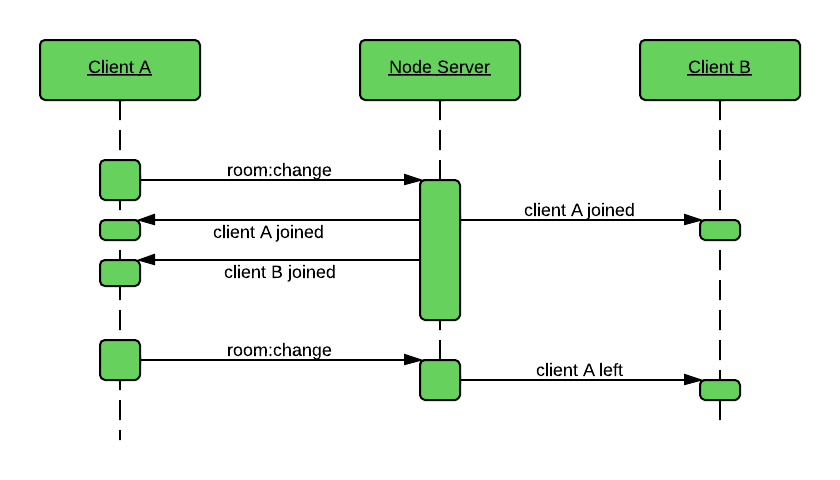
\includegraphics[width=15cm,keepaspectratio]{figures/join-seq.png}
\caption{Felhasználó belép a szobába}
\label{fig:joinseq}
\end{figure}

Az ábrán látszik, hogy szoba váltáskor a szerveroldal minden résztvevőjét a szobának (az új résztvevőt beleértve) értesít arról, hogy belépett, és az új résztvevőnek a létező socketek listáját is elküldi. Kilépéskor vagy diagram váltáskor is értesíti a klienseket. Így a kliensek nyilvántartást tudnak tartani a kapcsolódott többi kliensről. A \lstinline{client joined} és a \lstinline{client left} üzenetek esetében -- mivel az alkalmazás nem használ felhasználói fiókokat -- egy socket példány azonosítót is küld a kliensnek.

A socket azonosítókhoz színeket lehet nagyon egyszerűen rendelni úgy, hogy MD5 hasht számoltatok az azonosítóból és így egy hexadecimális értéket kapok. Ennek elég 6 betűjét venni és már megvan egy -- nagy valószínűséggel -- egyedi szín, legalábbis egy megnyitott diagramon belül.

Ez a jelölés a~\ref{fig:entitydir} ábrán is látszik. 

A jelöléseket egy kulcs-érték objektum tartalmazza, a kulcs az entitás azonosító, az érték az felhasználó színazonosítója. Ez a reláció irány azért hasznos, mert az entitás direktíva közvetlenül tud erre a színre hivatkozni:

\begin{lstlisting}
 <div class='entity_mark' style='background-color:#{{marks[entity._id]}};'>
 </div>
\end{lstlisting} 

tehát, ha van az objektumban egy konkrét entitás azonosító mint kulcs, akkor megjelenik egy olyan színű doboz, ha nem, akkor nem látszik semmi. 

Viszont, amikor egy másik kliens jelöléséről értesülünk, akkor egy entitás azonosítót és egy kliens azonosítót kapunk, ekkor nagyon kézenfekvő lenne a fordított irányú kulcs-érték objektum, vagyis kliens azonosítókhoz rendelt entitás azonosító. Ha ez meglenne, akkor egy műveletben kicserélnénk a régi jelölését az újra. Szerencsére az underscoreJS eszközkészletében találunk dictionary megfordítót:

\begin{lstlisting}
    socket.on('mark', function (data) {
        var inverted = _.invert($scope.marks)
        // user->id
        $scope.marks[inverted[data.user]] = null;
        $scope.marks[data.id] = data.user;
    });
\end{lstlisting}

Itt látszik, hogy ez a broadcast is szokásosan Socket.IO segítségével történik.